\documentclass[10pt,xcolor=dvipsnames]{beamer}
\usepackage[french]{babel}
\usepackage[utf8]{inputenc}
\usepackage[T1]{fontenc}
\usepackage{caption}
\usepackage{MnSymbol,wasysym}
\usepackage{amsmath}
\usepackage{cancel}
\usepackage[draft]{pdfcomment}
\newcommand{\pdfnote}[1]{\marginnote{\pdfcomment[icon=note]{#1}}}
\usepackage{appendixnumberbeamer}
\usepackage{comment}

\usepackage{pifont}% http://ctan.org/pkg/pifont
\newcommand{\cmark}{\textbf{\textcolor{darkspringgreen}{\ding{51}}}}%
\newcommand{\xmark}{\textbf{\textcolor{red}{\ding{55}}}}%

\usepackage{pgffor}

\renewcommand{\thefootnote}{\fnsymbol{footnote}}



\newcommand*\Let[2]{\State #1 $\gets$ #2}
\usepackage{algorithm}
\usepackage[noend]{algpseudocode}
\usepackage{tcolorbox}

\newtcolorbox{mybox}[3][]
{
  colframe = #2!25,
  colback  = #2!10,
  coltitle = #2!20!black,  
  title    = {#3},
  #1,
}

\usetheme[progressbar=frametitle,numbering=fraction]{metropolis}
%LS:
\setbeamercolor{background canvas}{bg=white}  
\usepackage{appendixnumberbeamer}

\usepackage{booktabs}
\usepackage[scale=2]{ccicons}
\usepackage{tikz}
\usetikzlibrary{calc}
\usepackage{color}
\usepackage{mathtools}

\usetikzlibrary{shapes,snakes}
%% Color Definition
\definecolor{darkspringgreen}{rgb}{0.09, 0.45, 0.27}
\definecolor{push}{HTML}{00AF37}
\definecolor{pull}{HTML}{3319BC}

\newcommand{\push}[1]{\textcolor{push}{push(#1)}}
\newcommand{\pull}[1]{\textcolor{pull}{pop(#1)}}
\newcommand{\pop}{\textcolor{pull}{pop()}}

\newcommand{\defin}[1]{\textcolor{darkspringgreen}{#1}}
\setbeamertemplate{frame footer}{Rohan Fossé}

\setbeamercolor{footline}{fg=gray}

\def\checkmark{\tikz\fill[scale=0.4,color=darkspringgreen](0,.35) -- (.25,0) -- (1,.7) -- (.25,.15) -- cycle;}
\usepackage{pgfplots}
\usepgfplotslibrary{dateplot}

\usepackage{eso-pic}
\usepackage{xspace}
\long\def\/*#1*/{}


\usepackage{tikz}

\usepackage{verbatim}
\usepackage{movie15}

\usepackage{animate}

\usetikzlibrary{arrows,shapes}
\pgfdeclarelayer{background}
\pgfsetlayers{background,main}

\title{
Algorithmique et structure de données
}
\subtitle{Algorithme glouton et arbre couvrant}

\date{\centering 10 Novembre 2021}
\author{\centering \bf Rohan Fossé}


\begin{document}

\maketitle


\section{Algorithmes gloutons}

\begin{frame}{Problème d'optimisation}
\begin{exampleblock}{Problème d'optimisation}
 Un problème d'optimisation a les caractéristiques suivantes :
    \begin{itemize}
        \item Une solution est un \defin{\textbf{sous-ensemble}} d'une des données du problème;
        \item Il existe en général plusieurs solutions \defin{\textbf{admissibles}};
        \item A chaque solution (admissible) est associée une \defin{\textbf{valeur}} (en général un coût ou un gain).
    \end{itemize}
    Le problème d'optimisation consiste en non seulement à trouver une solution admissible, mais à trouver une solution de valeur \defin{\textbf{minimale}} (pour un coût) ou \defin{\textbf{maximale}} pour un gain.
    
\end{exampleblock}
   
    \only<2>{
    \begin{exampleblock}{un exemple: rendu de monnaie}
    \begin{itemize}
        \item \textbf{Problème :} on dispose de pièces de valeurs $v_1, v_2, .., v_n$;
        \item \textbf{Solution :} une suite de (valeurs de) pièces ayant pour total S;
        \item \textbf{Meilleure solution :} celle utilisant le moins possible de pièces.
    \end{itemize}
    \end{exampleblock}
    }
\end{frame}


\begin{frame}{Algorithme gloutons}
Il s'agit d'une \textit{stratégie particulière} pour résoudre un problème d'optimisation.
    \begin{exampleblock}{Algorithme glouton}
    Un \defin{algorithme glouton} est un algorithme qui construit une solution:
    \begin{itemize}
        \item élément par élément \textbf{sans jamais revenir en arrière};
        \item en se basant sur des considérations locales.
    \end{itemize}
    \end{exampleblock}
    
    \only<2>{
    \begin{alertblock}{Attention}
    Il n'existe \alert{\textbf{pas toujours}} un algorithme glouton pour résoudre un problème d'optimisation.
    \end{alertblock}
    }
\end{frame}

\begin{frame}{Algorithme glouton pour le rendu de monnaie}
    \begin{alertblock}{Algorithme glouton}
    \begin{enumerate}
        \item Tant que S > 0;
        \item Choisir la pièce de plus grande valeur $v$ inférieur à $S$;
        \item Recommencer avec S - v.
    \end{enumerate}
    \end{alertblock}
\only<2->{

\begin{minipage}{0.5\textwidth}
\begin{exampleblock}{Exemple correct}
S=16 avec pièces de 10, 5, 2, 1:
\begin{itemize}
    \item 16 - 10 = 6
    \item 6 - 5 = 1
    \item 1 - 1 = 0
\end{itemize}
3 pièces
\end{exampleblock}
\end{minipage}\only<3>{\begin{minipage}{0.5\textwidth}
\begin{exampleblock}{Exemple incorrect}
S=16 avec pièces de 9, 8 et 1:
\begin{itemize}
    \item 16 - 9 = 7
    \item 7 - 1 = 6
    \item ...
\end{itemize}

8 pièces alors que 8 + 8 = 16 en 2 pièces
\end{exampleblock}
\end{minipage}
}
}
\end{frame}

\begin{frame}{Coloration d'un graphe à l'aide d'un algorithme glouton}
\begin{alertblock}{Idée de l'algorithme}
    On se donne un graphe G = ( V , E ).
Pour tout $v\in V$ :
\begin{itemize}
    \item  On regarde l'ensemble des couleurs déjà attribuées aux voisins de s.
    \item On en déduit le plus petit entier naturel qui n'appartient pas à cet ensemble.
    \item On attribue cette couleur à s. 
\end{itemize}
\end{alertblock}


\foreach \n in {0,...,6}{
\only<\n>{
\begin{figure}
    \centering
    \includegraphics[scale=0.40]{figures/CM3/color-greedy-\n.png}
\end{figure}
}
}

\end{frame}

\section{Rappel de l'algorithme de Dijsktra}

\begin{frame}{Algorithme de Dijsktra}
\foreach \n in {0,...,20}{
\only<\n>{
    \begin{figure}
        \centering
        \includegraphics[scale=0.42]{figures/CM4/djikstra/frame_\n_delay-0.25s.jpg}
        \label{fig:my_label}
    \end{figure}
}
}
\underline{Source:} \textit{https://themergedsort.com/?p=261}
\end{frame}

\begin{frame}{Problème avec Dijsktra}
Considérons le graphe suivant:
\begin{minipage}{0.5\textwidth}
\begin{figure}
    \centering
    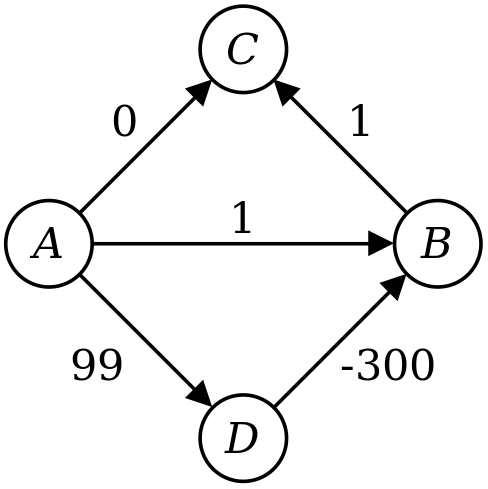
\includegraphics[scale=0.3]{figures/CM4/dji-neg.png}
    \label{fig:my_label}
\end{figure}
\end{minipage}\begin{minipage}{0.5\textwidth}
\begin{itemize}[<+->]
    \item   Tout d'abord, vous fixez d(A) à 0 et les autres distances à $\infty$.
    \item Vous développez ensuite le nœud A, en fixant d(B) à 1, d(C) à 0 et d(D) à 99.
    \item Ensuite, vous développez le nœud C;
    \item Vous développez ensuite le nœud B, ce qui n'a aucun effet.
    \item Enfin, vous développez D, ce qui fait passer d(B) à -201.
\end{itemize}
\end{minipage}

\end{frame}

\begin{frame}{Problème avec Dijsktra}
    Considérons le graphe suivant:
\begin{minipage}{0.5\textwidth}
\begin{figure}
    \centering
    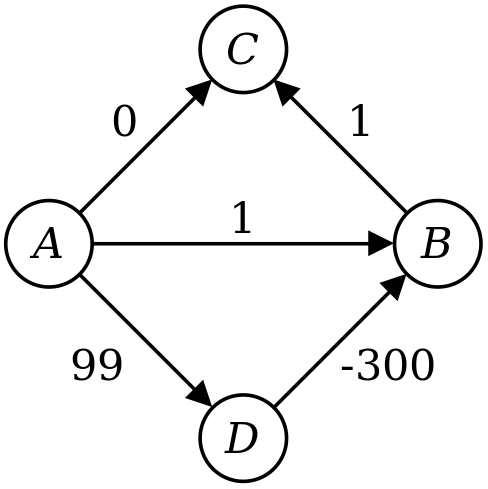
\includegraphics[scale=0.3]{figures/CM4/dji-neg.png}
    \label{fig:my_label}
\end{figure}
\end{minipage}\begin{minipage}{0.5\textwidth}
Remarquez cependant qu'à la fin, d(C) est toujours égal à 0, même si le plus court chemin vers C a une longueur de -200. Cela signifie que l'algorithme \alert{ne calcule pas} les distances correctes vers tous les nœuds.\\
De plus, même si vous stockez des pointeurs indiquant comment aller de chaque nœud au nœud de départ A, vous finirez par prendre le mauvais chemin de retour de C à A.
\end{minipage}
\end{frame}



\section{Algorithme de Bellman-Ford}
\begin{frame}{Algorithme de Bellman-Ford}
    \begin{exampleblock}{Histoire}
    L'algorithme de \alert{Bellman-Ford}  est un algorithme qui calcule des plus courts chemins depuis un sommet source donné dans un graphe orienté pondéré. Il porte le nom de ses inventeurs \textit{Richard Bellman} et \textit{Lester Randolph Ford junior}.
    \end{exampleblock}
    \only<2>{
    \begin{exampleblock}{Idée de l'algorithme}
    L'algorithme de Bellman-Ford permet de trouver le plus court chemin d'un sommet donné vers tous les autres sommets. De façon plus précise, à l'initialisation, chaque sommet à une étiquette initialisée à $\infty $ sauf le sommet qui a une étiquette à 0. Puis, à chaque itération , on calcule le plus court chemin de à tout autre sommet en au plus $k$ arcs.
    \end{exampleblock}
    }
\end{frame}

\begin{frame}{Déroulement sur un exemple}
    \begin{figure}
    \centering
    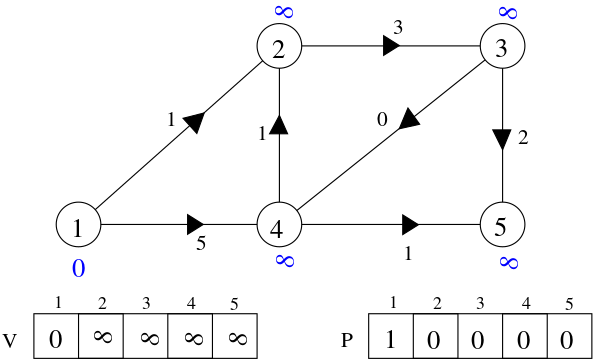
\includegraphics[scale=0.45]{figures/CM4/Bellman/Bellman0.png}
\end{figure}
\end{frame}


\begin{frame}{Déroulement sur un exemple}
\foreach \n in {0,...,12}{
\only<\n>{
\begin{figure}
    \centering
    \includegraphics[scale=0.45]{figures/CM4/Bellman/Bellman\n.png}
\end{figure}
}
}

\foreach \n in {13,...,14}{
\only<\n>{
\begin{figure}
    \centering
    \includegraphics[scale=0.37]{figures/CM4/Bellman/Bellman\n.png}
\end{figure}
}
}
\end{frame}

\begin{frame}{A vous de jouer !}

\begin{figure}
    \centering
    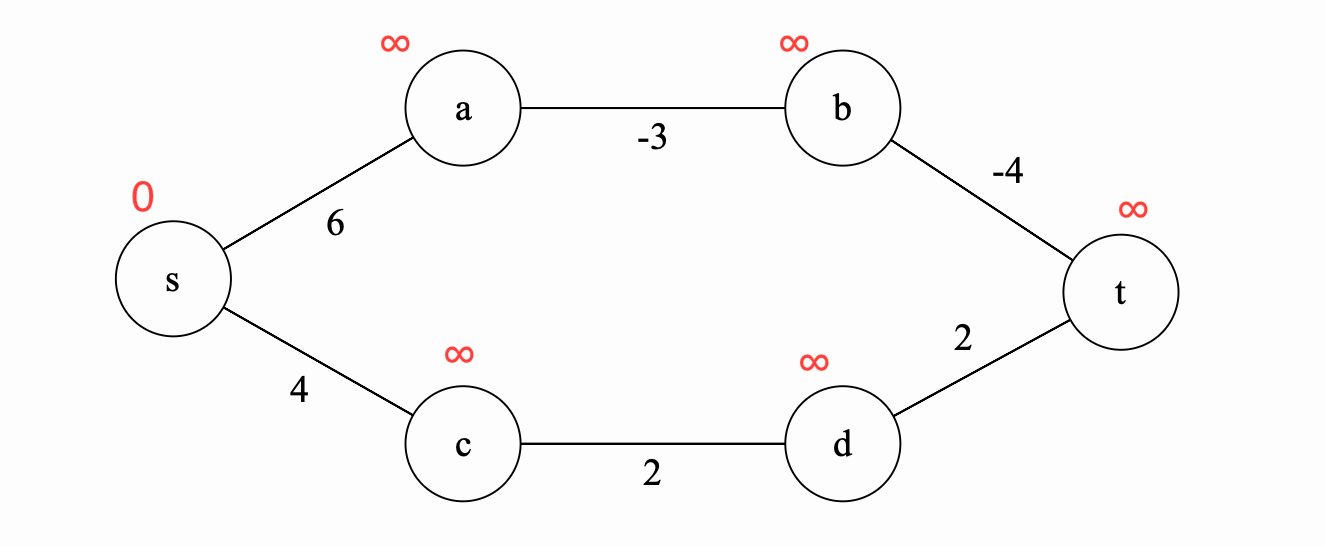
\includegraphics[scale=0.25]{figures/CM4/Bellman-2/i0.png}
\end{figure}

\end{frame}

\begin{frame}{A vous de jouer !}
    \foreach \n in {0,...,5}{
\only<\n>{
\begin{figure}
    \centering
    \includegraphics[scale=0.25]{figures/CM4/Bellman-2/i\n.png}
\end{figure}
}
}
\end{frame}


\section{Problème de l'arbre couvrant}

\begin{frame}{Rappel des définitions}
    \begin{exampleblock}{Arbre}
    un \defin{arbre} est un graphe connexe et sans cycle.
    \end{exampleblock}
    \only<2->{
    Attention, la notion est différente des arbres utilisés habituellement en algo:
    \begin{itemize}
        \item Aucune contrainte d'arité;
        \item Pas de notion de \alert{racine}
    \end{itemize}
    }
    \only<3>{
    \begin{alertblock}{Propriétés}
    \begin{itemize}
        \item Entre deux sommets donnés d'un \alert{arbre}, il existe toujours exactement une chaîne (élémentaire);
        \item Un arbre à $n$ sommets comporte $n - 1$ arêtes.
    \end{itemize}
    \end{alertblock}
    }
\end{frame}


\begin{frame}{Rappel des définitions}
    \begin{exampleblock}{Sous-graphe}
    Si G = (V, E), un sous-graphe de G est un graphe H = (V' ,E') avec
$V' \subseteq X$ et $E' \subseteq E$.
    \end{exampleblock}
    
    \only<1>{
    \begin{figure}
        \centering
        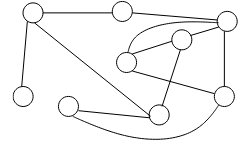
\includegraphics[scale=0.9]{figures/CM4/sous-graphe-1.png}
        \label{fig:my_label}
    \end{figure}
    }
        \only<2->{
    \begin{figure}
        \centering
        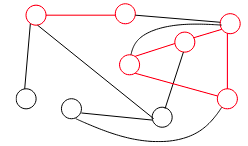
\includegraphics[scale=0.9]{figures/CM4/sous-graphe-2.png}
        \label{fig:my_label}
    \end{figure}
    \only<3>{
    Un sous-graphe de G est dit \alert{couvrant} s'il contient tous les sommets de G. Attention, un sous-graphe couvrant n'est pas forcément connexe.
    }
    }
\end{frame}

\begin{frame}{Arbre couvrant}
    Tout graphe connexe admet un \alert{arbre couvrant}.
    
    \only<1>{
    \begin{figure}
        \centering
        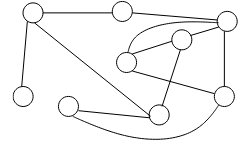
\includegraphics[scale=0.9]{figures/CM4/sous-graphe-1.png}
        \label{fig:my_label}
    \end{figure}
    }
        \only<2->{
    \begin{figure}
        \centering
        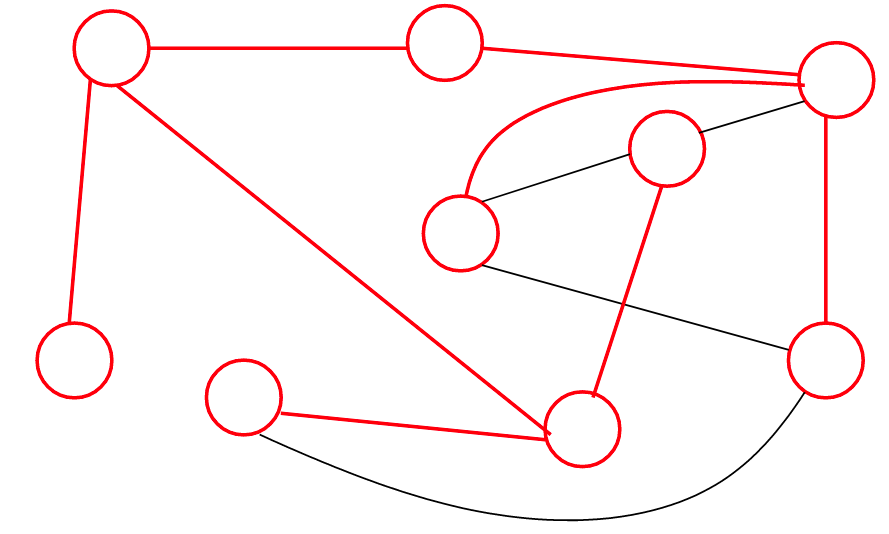
\includegraphics[scale=0.25]{figures/CM4/couvrant-1.png}
        \label{fig:my_label}
    \end{figure}
    }
\end{frame}

\begin{frame}{Caractérisation d'un arbre couvrant}
    \begin{figure}
        \centering
        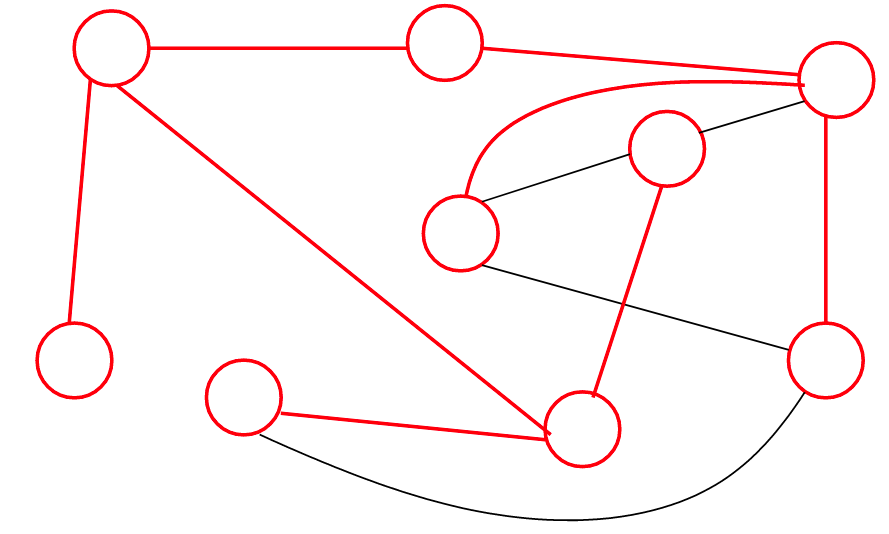
\includegraphics[scale=0.10]{figures/CM4/couvrant-1.png}
        \label{fig:my_label}
    \end{figure}
Si A est un sous-graphe couvrant d'un graphe G ayant V sommets, les caractérisations suivantes sont \alert{équivalentes}:
\begin{itemize}
    \item A est un \alert{arbre couvrant} de G;
    \item A est sans cycle et possède V - 1 arêtes;
    \item A est \alert{connexe}
    \item On ne peut pas ajouter une arête à A sans créer un \alert{cycle};
    \item On ne peut pas retirer une arête à A sans briser sa \alert{connexité}.
\end{itemize}
\end{frame}

\begin{frame}{Dans un graphe pondéré}
\begin{alertblock}{Arbre couvrant de poids minimal}
Le poids d'un sous-graphe est la somme des poids des arêtes. Nous cherchons un \alert{arbre couvrant de poids minimal} (en anglais \textit{Minimum Spanning Tree} (MST) )
\end{alertblock}


\only<1>{
    \begin{figure}
        \centering
        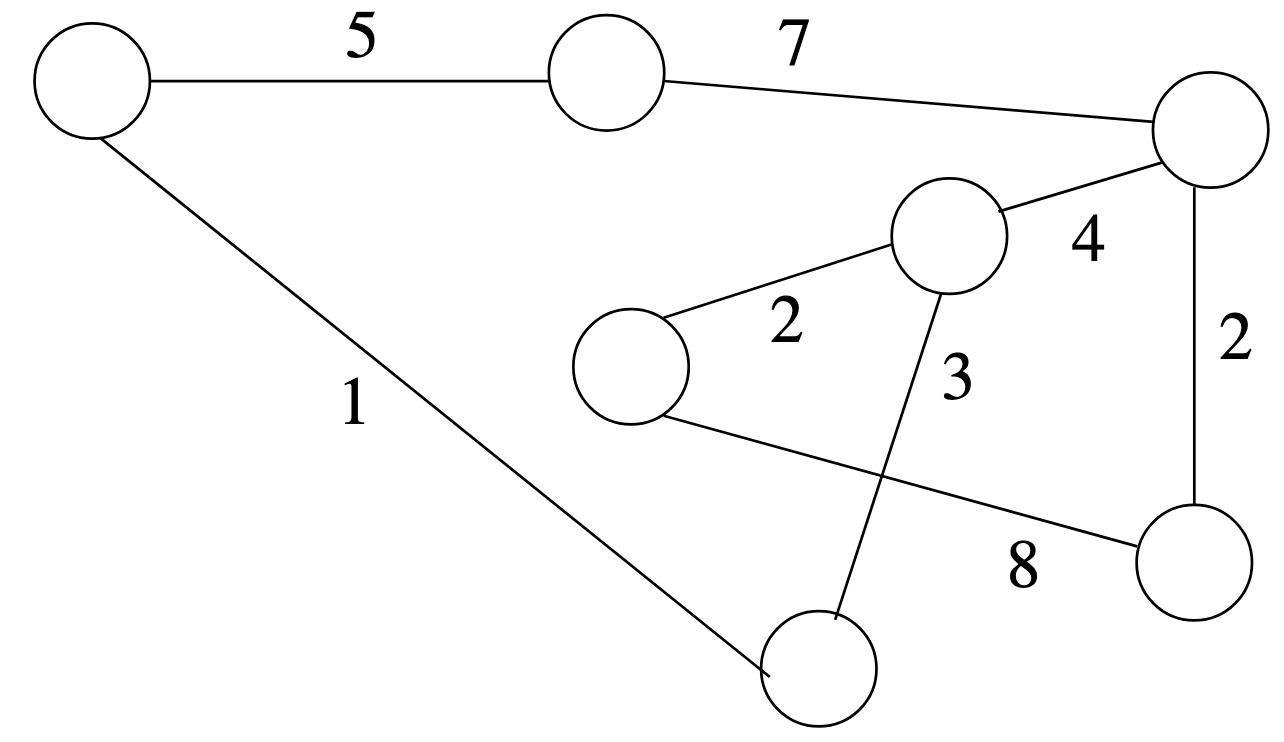
\includegraphics[scale=0.18]{figures/CM4/MST-1.png}
        \label{fig:my_label}
    \end{figure}
    }
    \only<2>{
    
        \begin{figure}
        \centering
        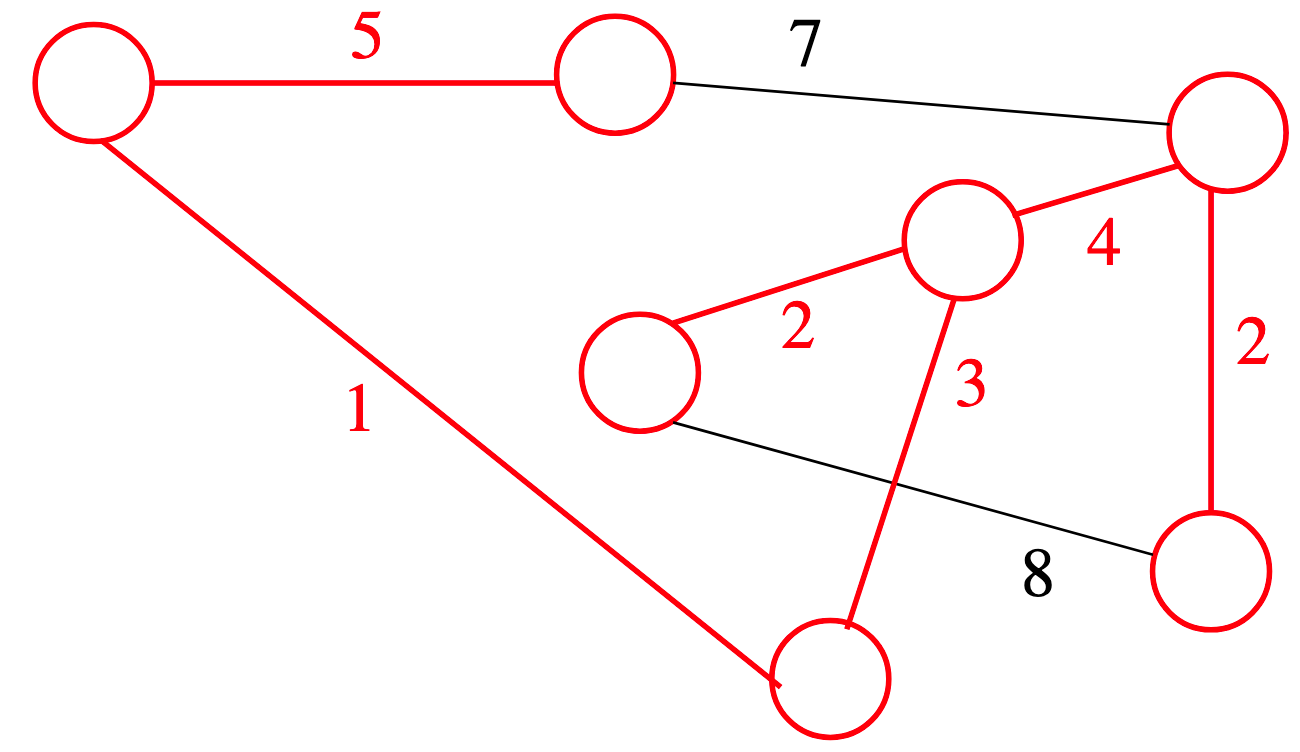
\includegraphics[scale=0.18]{figures/CM4/MST-2.png}
        \label{fig:my_label}
    \end{figure}
    }
\end{frame}

\begin{frame}{Application}
\begin{exampleblock}{Problème}
    

    Problème proposé (et résolu) en 1926 par \textit{Otakar Boruvka} pour la construction de réseaux électriques efficaces.
    
    \begin{itemize}
        \item Les sommets de G représentent des lieux à connecter: villes, ordinateurs, composants électroniques, etc.
        \item Les arêtes de G représentent les liens (routes, câbles,..) \alert{possibles} entre ces lieux, avec les coûts effectifs de création de ces liens.
        \item L'arbre couvrant minimal est le réseau le moins coûteux ne laissant aucun lieu isolé.
    \end{itemize}
\end{exampleblock}
\only<2>{
\textbf{Attention}: on minimise le coût global du réseau, pas les longeurs des chemins dans l'arbre.
Il existe des variantes du problème contraignant la forme de l'arbre obtenu: degré borné pour chaque sommet, diamètre borné, etc..
}
\end{frame}

\section{Algorithmes de détermination d'un arbre couvrant}


\begin{frame}{Algorithmes de détermination d'un arbre couvrant}

Deux idées duales:

    \begin{minipage}{0.5\textwidth}
\begin{exampleblock}{Première idée}
\only<1->{ A = (V,$\emptyset$) (\defin{le graphe vide)}\\ }
\only<2->{ 
\textbf{tant que}\\
\textbf{faire}\\
 \only<3->{Choisir une arête de \defin{G} qui ne \defin{crée pas de cycle.}}\\
 \defin{Ajouter cette arête à A}
}
\end{exampleblock}
\end{minipage}\begin{minipage}{0.5\textwidth}
\begin{exampleblock}{Deuxième idée}
\only<1->{ A = (V,E) (\defin{le graphe G)}\\ }
\only<2->{ 
\textbf{tant que}\\
\textbf{faire}\\
 \only<3->{Choisir une arête de \defin{A} qui n'est pas \defin{indispensable à la connexité}}\\
 \defin{Retirer cette arête de A}
}
\end{exampleblock}
\end{minipage}
    
 \only<4->{
Par construction, le graphe A obtenu est un arbre couvrant (en supposant que G soit connexe).
}
\only<5->{
\begin{exampleblock}{Critères de choix}
\begin{itemize}
\item \underline{Ne pas créer de cycle:} assez facile;
\item \underline{vérifier la connexité:} moins facile et plus coûteux dans le cas général.
\end{itemize}
\end{exampleblock}
}   
    
\end{frame}


\begin{frame}{Choisir une arête}
    Toute arête qui ne crée pas de cycle convient. Pour que l'arbre soit minimal, il faut aussi tenir compte des poids.\\
    La encore, deux choix sont possibles :
    \only<2->{
    \begin{alertblock}{Connexité d'abord : Algorithme de \alert{Prim}}
    On choisit l'arête de poids minimal \textbf{parmi celles incidentes à } A.\\
    En cours d'algorithme A est un \alert{arbre}. il suffit qu'une extrémité de l'arête choisie hors de A.
    \end{alertblock}
    }
    \only<3->{
    \begin{alertblock}{Minimalité d'abord: Algorithme de \textbf{Kruskal}}
    On choisit l’arête de poids minimal dans \alert{tout le graphe}. En cours d’algorithme A est une \textbf{forêt}.\\
    Il faut mémoriser si deux sommets sont dans des composantes
    connexes distinctes.
    \end{alertblock}
    }
    \only<4->{
    \alert{\begin{center}
        Utilisation des algorithmes gloutons
    \end{center}}
    }
\end{frame}


\section{Algorithme de Prim}

\begin{frame}{Algorithme de Prim}
\begin{exampleblock}{Histoire}
        L'algorithme a été développé en 1930 par le mathématicien tchèque \textit{Vojtech Jarnik}, puis a été redécouvert et republié par \textit{Robert C. Prim} et \textit{Edsger W. Dijkstra} en 1959.
\end{exampleblock}
\begin{figure}
    \centering
    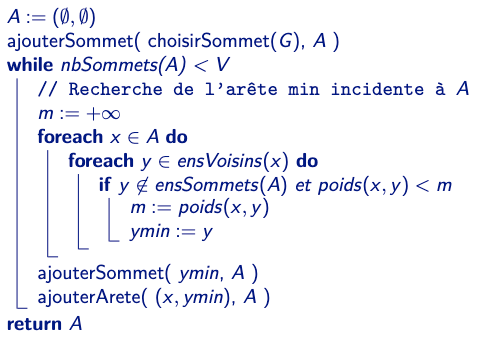
\includegraphics[scale=0.45]{figures/CM4/prim-algorithm.png}
    \label{fig:my_label}
\end{figure}
\end{frame}


\begin{frame}{Déroulement sur un exemple}

%% Adjacency matrix of graph
%% \  a  b  c  d  e  f  g
%% a  x  7     5
%% b  7  x  8  9  7
%% c     8  x     5
%% d  5  9     x 15  6
%% e     7  5 15  x  8  9
%% f           6  8  x 11
%% g              9  11 x

\tikzstyle{vertex}=[circle,fill=black!25,minimum size=20pt,inner sep=0pt]
\tikzstyle{selected vertex} = [vertex, fill=red!24]
\tikzstyle{edge} = [draw,thick,-]
\tikzstyle{weight} = [font=\small]
\tikzstyle{selected edge} = [draw,line width=5pt,-,red!50]
\tikzstyle{ignored edge} = [draw,line width=5pt,-,black!20]

\begin{figure}
\begin{tikzpicture}[scale=1.8, auto,swap]
    % Draw a 7,11 network
    % First we draw the vertices
    \foreach \pos/\name in {{(0,2)/a}, {(2,1)/b}, {(4,1)/c},
                            {(0,0)/d}, {(3,0)/e}, {(2,-1)/f}, {(4,-1)/g}}
        \node[vertex] (\name) at \pos {$\name$};
    % Connect vertices with edges and draw weights
    \foreach \source/ \dest /\weight in {b/a/7, c/b/8,d/a/5,d/b/9,
                                         e/b/7, e/c/5,e/d/15,
                                         f/d/6,f/e/8,
                                         g/e/9,g/f/11}
        \path[edge] (\source) -- node[weight] {$\weight$} (\dest);
    % Start animating the vertex and edge selection. 
    \foreach \vertex / \fr in {d/1,a/2,f/3,b/4,e/5,c/6,g/7}
        \path<\fr-> node[selected vertex] at (\vertex) {$\vertex$};
    % For convenience we use a background layer to highlight edges
    % This way we don't have to worry about the highlighting covering
    % weight labels. 
    \begin{pgfonlayer}{background}
        \pause
        \foreach \source / \dest in {d/a,d/f,a/b,b/e,e/c,e/g}
            \path<+->[selected edge] (\source.center) -- (\dest.center);
        \foreach \source / \dest / \fr in {d/b/4,d/e/5,e/f/5,b/c/6,f/g/7}
            \path<\fr->[ignored edge] (\source.center) -- (\dest.center);
    \end{pgfonlayer}
\end{tikzpicture}
\end{figure}
\end{frame}

\begin{frame}{Caractère glouton}
    On retrouve les caractéristiques d'un algorithme glouton :
    \begin{itemize}
        \item La solution construite est un ensemble (d'arêtes);
        \item Les solutions admissibles sont les arbres couvrants;
        \item On recherche une solution de poids total minimal;
        \item L'algorithme de Prim procède uniquement par ajout d'arêtes (et de sommets) dans A;
        \item Le choix de la prochaine arête n'est basé que sur son poids.
    \end{itemize}
    
    L'algorithme a donc coût en $\mathcal{O}(V \times C$ où $C$ est le coût du choix de la prochaine arête.
\end{frame}

\begin{frame}{A vous de jouer !}

\begin{figure}
    \centering
    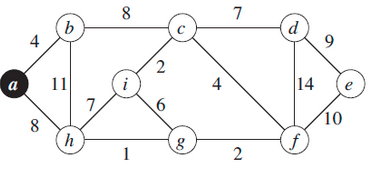
\includegraphics[scale=0.8]{figures/CM4/Prim-2/i0.png}
\end{figure}

\end{frame}

\begin{frame}{A vous de jouer !}
    \foreach \n in {0,...,9}{
\only<\n>{
\begin{figure}
    \centering
    \includegraphics[scale=0.8]{figures/CM4/Prim-2/i\n.png}
\end{figure}
}
}
\end{frame}
\section{Algorithme de Kruskal}

\begin{frame}{Algorithme de Kruskal}
    \begin{exampleblock}{Algorithme}
    L'algorithme construit un \alert{arbre couvrant minimum} en sélectionnant des arêtes par poids croissant.\\
    Plus précisément, l'algorithme considère toutes les arêtes du graphe par \alert{poids croissant} (en pratique, on trie d'abord les arêtes du graphe par poids croissant) et pour chacune d'elles, il la sélectionne si elle ne crée pas un \alert{cycle}. 
    \end{exampleblock}
    \only<2>{
    \begin{figure}
        \centering
        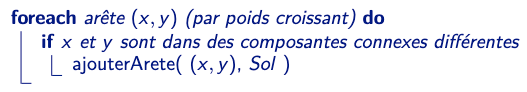
\includegraphics[scale=0.5]{figures/CM4/Krusal-algo.png}
        \label{fig:my_label}
    \end{figure}
    }
\end{frame}

\begin{frame}{Déroulement sur un exemple}
    \foreach \n in {0,...,39}{
\only<\n>{
    \begin{figure}
        \centering
        \includegraphics[scale=0.40]{figures/CM4/Kruskal/frame_\n_delay-0.5s.jpg}
        \label{fig:my_label}
    \end{figure}
}
}
\end{frame}


\begin{frame}{Conclusion du cours}
    \begin{itemize}
        \item Présentation des algorithmes gloutons;
        \item Faiblesse de l'algorithme de Dijsktra et algorithme de Bellman-Ford;
        \item Définition d'un arbre couvrant;
        \item Algorithme de Prim;
        \item Algorithme de Kruskal.
    \end{itemize}
\end{frame}

\end{document}